%第2章:準備
本章では本文中に使用する用語、実験環境およびシステム概要について述べる

\section{諸定義}

\subsection*{V字モデル}
V字モデルとはシステム開発を要求分析、基本設計、詳細設計、実装に分け上から順にそれぞれに対して検証、テストを行いながら上から順に時間軸に従って行っていく。細かく要素ごとにテストをしていくことで開発の途中で大幅な変更や問題が起きにくくなる利点がある。

\begin{figure}[htbp]
\centering
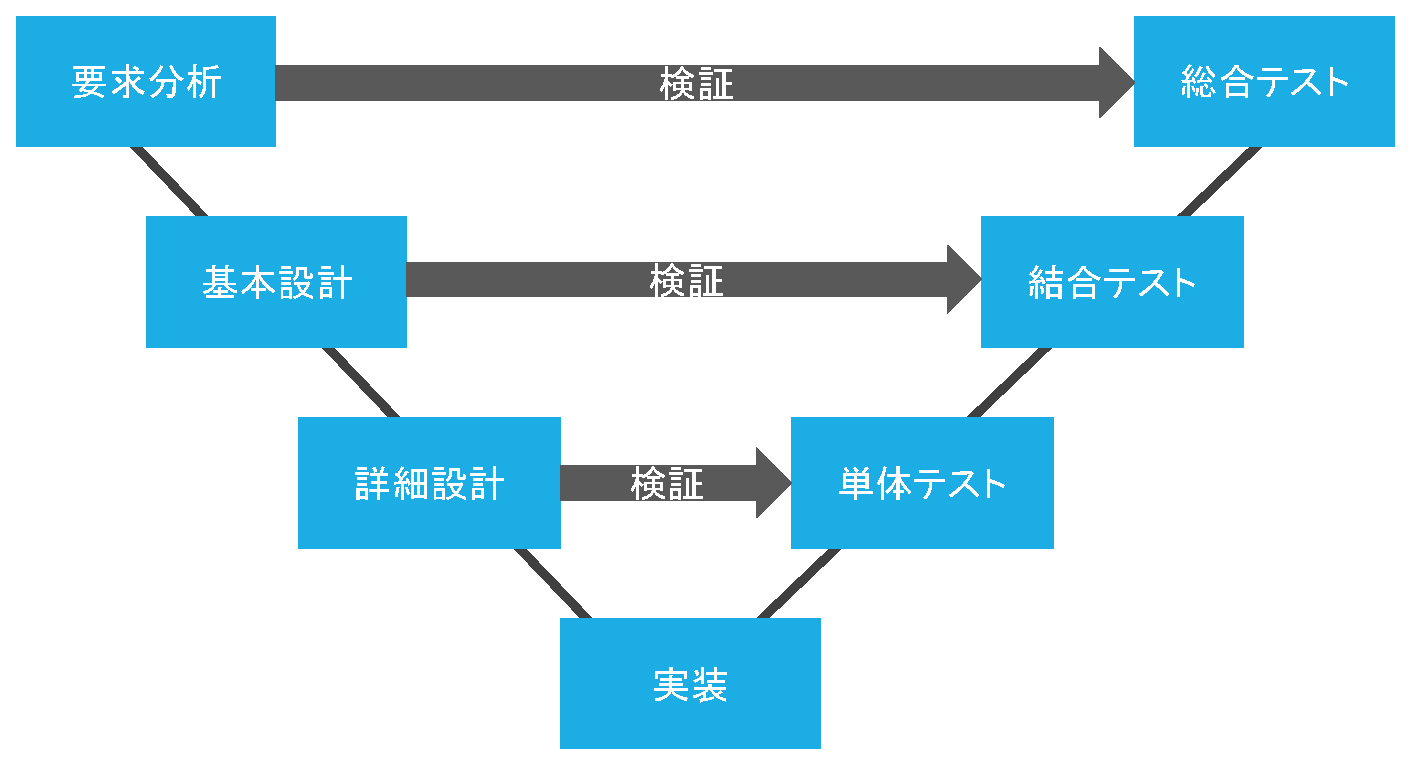
\includegraphics[width=12cm]{./pic/vjimodel.eps}
\caption{V字モデル}
\label{v_model}
\end{figure}

\subsection*{UML(Unifiled Modeling Language)}
UMLとは各開発工程で利用すべき図面の標準化されたモデルである。UMLで一番重視されていることは、単純で分かりやすいという軸と十分実用に使えるだけの強力な表現方法を持つ軸を最適に組み合わせて言語設計をすることである。UMLの構成要素としてユースケース図、クラス図、シーケンス図がある。\cite{uml}

\subsection*{ユースケース図}
システムがどのように機能すべきかという振る舞いとその外部環境を表す。


\subsection*{シーケンス図}
シーケンス図は、オブジェクト間のメッセージのやり取りを時系列順に沿って並べて表現したもの。
ユースケース図を基にしてシーケンス図やクラス図を制作していく。

\subsection*{クラス図}
クラス図はモデルの静的な構造を示す図。クラスが持つ動作や、属性を記述する。より具体的な実装部分に近い記述をしていく。

\subsection*{Yolo(Real-Time Object Detection)}
Yoloはリアルタイムでのオブジェクト識別が可能なネットワークを目的としている。Webカメラでのリアルタイム検出を行うこともできるFPSを誇る。ほかのネットワークとの違いは検出と、識別を同時に行っているため高速性を保てる点である。今回は画像からバーコードの位置を特定するために使用した。\cite{yolo}.


\subsection*{pyzbar}
バーコード画像データを解析して数字を識別するライブラリである。\cite{pyzbar}.

\section{システムの概要}
 システムでは、買い物かごにエッジ処理を担当するRaspberryPiと各種センサを設置する。エッジ側では商品の特定に必要となるデータをセンサ類を用いて取得する。データを取得したらサーバ側に送信し、そこで画像データを処理して商品の特定を行う。システムの流れを以下の図に示す。

すべての機能を実装するには時間の問題から難しいと判断したので赤枠で囲った部分のみを行った。


\section{実験環境}
 実験環境で使用したものを以下の表に示す。

\begin{table}[htb]
\begin{center}
\caption{実行環境}
\begin{tabular}{|c|c|c|c|c|} \hline
処理担当 & OS & CPU & RAM & GPU \\ \hline
サーバ側 & Windows10 64bit Pro & Core2Duo & 4GB & GT740 \\ \hline
エッジ側 & RaspberryPi3B+(Rasbian) & 1.2GHz & 1GB & None \\ \hline
\end{tabular}
\label{spec}
	\end{center}
\end{table}


